\documentclass[12pt]{article}
\usepackage{vntex}
% \usepackage[english, vietnamese]{babel}
\usepackage{tikz}
\usepackage[left=3.00cm, right=2.00cm, top=2.00cm, bottom=2.00cm]{geometry}
\usepackage[unicode]{hyperref}
\usepackage{amsmath}
\usepackage{amssymb}
\usepackage{graphicx}
\usepackage{a4wide,amssymb,epsfig,latexsym,array,hhline,fancyhdr}
\usepackage[normalem]{ulem}
\usepackage[makeroom]{cancel}
\usepackage{amsthm}
\usepackage{multicol,longtable,amscd}
\usepackage{diagbox}
\usepackage{booktabs}
\usepackage{alltt}
\usepackage[framemethod=tikz]{mdframed}
\usepackage{caption,subcaption}
\usepackage{listings}
\usepackage{color}
\usepackage{lipsum}
\usepackage{setspace}
\usepackage{titling}
\usepackage{multicol}
\usepackage{indentfirst}
\usepackage{float}

\usetikzlibrary{decorations}
\usetikzlibrary{decorations.pathreplacing}
\usetikzlibrary{decorations.pathreplacing,calligraphy}
\usetikzlibrary{arrows.meta}
\usetikzlibrary{calc}

\setstretch{1}

\newtheorem*{theorem}{Định lý}
\newtheorem{corollary}{Hệ quả}
\newtheorem{lemma}{Bổ đề}
\newtheorem*{remark}{Nhận xét}
\newtheorem{definition}{Định nghĩa}
\newtheorem*{recap}{Tóm lại}


\title{\textbf{Kuratowski's Theorem}}
\posttitle{
\par\end{center}
\begin{center}\LARGE(Toán rời rạc)\end{center}
\vskip0.5em}



\author{
    Nguyễn Đức Huy \thanks{K64 ...}\\
    Departement \\
    Đại học Khoa học Tự Nhiên \\
    mail@edu
    \and
    Trần Thị Như Quỳnh \thanks{K65 ...} \\
    Departement \\
    Đại học Khoa học Tự Nhiên \\
    mail@edu
    \and
    Bùi Khánh Duy \thanks{K65 ...}\\
    Departement \\
    Đại học Khoa học Tự Nhiên \\
    mail@edu
}

\begin{document}
\begin{titlepage}
    \maketitle
    \begin{abstract}
        Đây là tóm tắt \footnote{Quyền sao chép một phần hoặc toàn bộ bài viết này cho mục đích sử dụng cá nhân hoặc lớp học được cho phép với điều kiện bản sao không được tạo ra hoặc phân phối vì lợi nhuận hoặc mục đích thương mại và các bản sao đó phải trích dẫn đầy đủ thông báo này trên trang đầu tiên. Các bên thứ ba của bài viết này phải được tôn trọng. Đối với tất cả các mục đích sử dụng khác, hãy liên hệ với chủ sở hữu hoặc các tác giả}
    \end{abstract}
\end{titlepage}

\begin{titlepage}
    \tableofcontents
\end{titlepage}

\section{Mở đầu}

Đôi lời phát biểu, thêm sau

\textcolor{blue}{\section{Classical Cryptography}}
Một trong những người sử dụng mật mã được biết đến sớm nhất là Julius Caesar.
Ông đã làm cho các thông điệp trở nên bí mật bằng cách \textit{dịch chuyển} mỗi chữ cái đi ba chữ
cái về phía trước trong bảng chữ cái \thanks{Bảng chữ cái ở đây là bảng chữ cái tiếng Anh, các ví dụ cũng được giữ nguyên gốc} (và ba chữ cái cuối cùng của bảng chữ cái
thành ba chữ cái đầu tiên). Ví dụ, theo sơ đồ này, chữ B được chuyển thành E và
chữ X được chuyển thành A. Đây là một ví dụ về mã hóa, tức là quá trình tạo một thông
điệp bí mật.

Để biểu diễn quy trình mã hóa của Caesar theo toán học, trước tiên
hãy thay thế mỗi chữ cái bằng một phần tử của $ \mathbf{Z}_{26} $, nghĩa là một số nguyên từ 0
đến 25 dựa trên vị trí của nó trong bảng chữ cái. Ví dụ, thay A bằng 0,
K bằng 10 và Z bằng 25. Phương pháp mã hóa của Caesar có thể được biểu diễn bằng
hàm $f$ tác động vào số nguyên không âm $p$, $0 \leq p \leq  25$, số nguyên $f(p)$ trong tập
$\{0, 1, 2, \ldots, 25\}$ sao cho:
$$f(p) = (p+3)\ \mathbf{mod}\ 26$$
Như vậy, trong phiên bản đã được mã hóa của thông điệp, chữ cái được biểu diễn bởi $p$ sẽ được thay thế bằng
chữ cái được biểu diễn bởi $(p+3)\ \mathbf{mod}\ 26$
\begin{example}
    Thông điệp mã hóa của thông điệp "MEET YOU IN THE PARK" sử dụng cách mã hóa Caesar là gì?
\end{example}
\begin{solution}
    Trước tiên, ta thay các chữ cái trong thông điệp bởi các số tương ứng, ta được:
    \begin{center}
        12 4 4 19 \hspace{0.5cm} 24 14 20 \hspace{0.5cm} 8 13 \hspace{0.5cm} 19 7 4 \hspace{0.5cm} 15 0 17 10
    \end{center}
    Tiếp theo, ta thay mỗi số $p$ bởi $f(p) = (p+3)\ \mathbf{mod}\ 26$, ta được:
    \begin{center}
        15 7 7 22 \hspace{0.5cm} 1 17 23 \hspace{0.5cm} 11 16 \hspace{0.5cm} 22 10 7 \hspace{0.5cm} 18 3 20 13
    \end{center}
    Với mỗi số, ta thay ngược lại bởi các chữ cái tương ứng, ta thu được thông điệp được mã hóa "PHHW BRX LQ WKH SDUN".
\end{solution}
Để phục hồi lại thông điệp gốc đã được mã hóa theo cách mã hóa Caesar, ta cần phải dùng hàm ngược $f^{-1}$ của hàm $f$.
Chú ý hàm $f^{-1}$ ánh xạ số nguyên $p$ từ tập $ \mathbf{Z}_{26} $, đến $f^{-1}(p) = (p-3)\ \mathbf{mod}\ 26$.
Nói cách khác, để tìm được thông điệp gốc, mỗi chữ cái được \textit{dịch chuyển} ba chữ
cái về phía sau trong bảng chữ cái, với ba chữ cái đầu tiên được chuyển thành ba chữ cái cuối
cùng. Quá trình xác định thông điệp gốc từ thông điệp được mã
hóa được gọi là \textbf{giải mã}.

Có nhiều cách khác nhau để khái quát cách mã hóa Caesar. Ví dụ, thay vì \textit{dịch chuyển} mỗi chữ cái cho 3,
ta có thể \textit{dịch chuyển} mỗi chữ cái cho $k$ chữ cái về phía trước, tức là:
$$f(p) = (p+k)\ \mathbf{mod}\ 26$$
Một mật mã như thế được gọi là \textbf{mật mã dịch}. Đối với loại mật mã này, việc giải mã thực hiện bằng cách dùng
$$f^{-1}(p) = (p-k)\ \mathbf{mod}\ 26$$
Ở đây số nguyên $k$ được gọi là \textbf{khóa}. Chúng tôi minh họa việc sử dụng mật mã dịch trong Ví dụ 2 và 3.
\begin{example}
    Mã hóa văn bản thông báo “STOP GLOBAL WARMING” bằng cách sử dụng mật mã dịch với khóa $k = 11$
\end{example}
\begin{solution}
    Để mã hóa thông điệp “STOP GLOBAL WARMING”, trước tiên ta thay các chữ cái trong thông điệp bởi các số tương ứng trong $ \mathbf{Z}_{26} $. Điều này tạo ra chuỗi
    \begin{center}
        18 19 14 15 \hspace{0.5cm} 6 11 14 1 0 11 \hspace{0.5cm} 22 0 17 12 8 13 6
    \end{center}
    Bây giờ ta áp dụng hàm dịch $f(p) = (p+k)\ \mathbf{mod}\ 26$ cho mỗi số trong chuỗi này. Ta thu được
    \begin{center}
        3 4 25 0 \hspace{0.5cm} 17 22 25 12 11 22 \hspace{0.5cm} 7 11 2 23 19 24 17
    \end{center}
    Thay thế chuỗi cuối cùng này trở lại các chữ cái, ta thu được thông điệp mã hóa
    "DEZA RWZMLW HLCXTYR".
\end{solution}
\begin{example}
    Giải mã thông điệp mật mã "LEWLYPLUJL PZ H NYLHA ALHJOLY" đã được mã
    hóa bằng mật mã dịch với khóa $k = 7$.
\end{example}
\begin{solution}
    Để giải mã thông điệp "LEWLYPLUJL PZ H NYLHA ALHJOLY", trước tiên ta
    thay các chữ cái bởi các phần tử tương ứng trong $ \mathbf{Z}_{26} $. Ta đạt được
    \begin{center}
        11 4 22 11 24 15 11 20 9 11 \hspace{0.5cm} 15 25 \hspace{0.5cm} 7 \hspace{0.5cm} 13 24 11 7 0 \hspace{0.5cm} 0 11 7 9 14 11 24
    \end{center}
    Để giải mã, ta phải dùng hàm $f^{-1}(p) = (p-7)\ \mathbf{mod}\ 26$, áp dụng cho mỗi số trong chuỗi, ta được
    \begin{center}
        4 23 15 4 17 8 4 13 2 4 \hspace{0.5cm} 8 18 \hspace{0.5cm} 0 \hspace{0.5cm} 6 17 4 0 19 \hspace{0.5cm}  19 4 0 2 7 4 17
    \end{center}
    Cuối cùng, ta thay thế các số này trở lại thành các chữ cái để thu được thông điệp gốc. Ta thu được "EXPERIENCE IS A GREAT TEACHER".
\end{solution}

Rõ ràng, phương pháp của Caesar và mật mã dịch không có độ an toàn cao.
Ta có thể tổng quát hóa mật mã dịch để tăng cường độ bảo mật
bằng cách sử dụng hàm
$$f(p) = (ap+b)\ \mathbf{mod}\ 26$$
trong đó $a$ và $b$ là các số nguyên sao cho thỏa mãn $f$ là song ánh ($f(p)$ là song ánh khi và chỉ khi
UCLN$(a,26)$ = 1). Một hàm như vậy được gọi là \textbf{hàm tuyến tính} và mật mã dịch thu được sau khi dùng hàm tuyến tính là \textbf{mật mã dich tuyến tính}.
\begin{example}
    Chữ cái nào thay thế cho chữ K khi dùng hàm $f(p) = (7p + 3)\ \textbf{mod}\ 26$ để mã hóa?
\end{example}
\begin{solution}
    Đầu tiên, ta biết rằng số 10 tương ứng cho chữ K. Sau đó, dùng hàm mã hóa
    $f(p)$, ta được $f (10) = (7 \times 10 + 3)\ \textbf{mod}\ 26 = 21$. Bởi vì 21 tương ứng
    với chữ V, vậy nên sẽ K được thay thế bằng V trong thông điệp mã hóa.
\end{solution}
\textcolor{blue}{\section{Hệ mã hóa khóa công khai}}
Tất cả các mật mã cổ điển, bao gồm mật mã dịch và mật mã dịch tuyến tính, là những ví dụ về \textbf{hệ mã hóa khóa bí mật}. Trong hệ mã hóa khóa bí mật, một khi đã biết khóa, bạn có thể nhanh chóng giải mã. Vì vậy, biết cách mã hóa bằng một khóa cụ thể cho phép giải mã các thông điệp đã được mã hóa bằng khóa này. Ví dụ, khi mã hóa bằng mật mã dịch với khóa k, số nguyên $p$ sẽ trở thành
$$c = (p+k)\ \mathbf{mod}\ 26$$
Còn việc giải mã $c$ sẽ trở thành
$$p = (c-k)\ \mathbf{mod}\ 26$$
Vậy, khi biết cách mã hóa, ta sẽ biết cách giải mã.

Khi dùng mã hóa khóa bí mật, hai bên muốn giao tiếp bí mật phải dùng chung khóa.
Bởi vì bất kỳ ai biết khóa này đều có thể mã hóa và giải mã thông điệp, hai người muốn giao tiếp bí mật phải trao đổi khóa một cách an toàn.
(Tôi sẽ giới thiệu một phương pháp để thực hiện việc này ở phần sau.)
Mật mã dịch và mật mã dịch tuyến tính thuộc loại mã hóa khóa bí mật. Chúng khá đơn giản và cực kỳ dễ bị phá.
Tuy nhiên, điều này không đúng với tất cả các mật mã thuộc loại mã hóa khóa bí mật.
Đặc biệt, tiêu chuẩn của chính phủ Hoa Kỳ về mã hóa khóa bí mật, được gọi là tiêu chuẩn mã hóa tiên tiến (AES), cực kỳ
phức tạp và được coi là có tính bảo mật cao (khó bị phá).
AES được sử dụng rộng rãi trong thương mại và chính phủ.
Để tăng cường bảo mật, mỗi khóa mới được sử dụng cho một phiên giao tiếp giữa hai bên, điều này yêu cầu phương pháp tạo khóa và gửi khóa một cách an toàn.

Để tránh việc phải chia sẻ khóa mỗi phiên giao tiếp, vào những năm 1970, các nhà mật mã học đã đưa ra khái niệm về \textbf{hệ mã hóa khóa công khai}.
Khi sử dụng mã hóa khóa công khai, chỉ biết mã hóa thông điệp không giúp ta giải mã được. Tất cả mọi người đều có thể biết khóa công khai.
Chỉ duy nhất khóa dùng để giải mã được giữ bí mật và chỉ người nhận thông điệp mới có thể giải mã nó,
vì theo những gì được biết hiện nay, nếu chỉ biết cách mã hóa thì việc giải mã không hề dễ dàng.

Hệ mã hóa khóa công khai đầu tiên được phát minh vào khoảng giữa những năm 1970. Trong những thập kỷ tiếp theo,
nhiều hệ mã hóa khóa công khai khác cũng được ra đời. Ở phần dưới, tôi sẽ giới thiệu một hệ mã hóa khóa công khai được sử dụng phổ biến nhất, được gọi là hệ RSA.
Bên cạnh hệ RSA, có nhiều hệ mã hóa khóa công khai khác có nhiều ứng dụng trong thời điểm hiện nay.
Các hệ mã hóa khóa công khai này sẽ đóng một vai trò quan trọng khi những tiến bộ trong việc giao tiếp có thể làm cho hệ mã hóa RSA trở nên lỗi thời, điều này thường xảy ra trong mật mã học.

Mặc dù mã hóa khóa công khai có ưu điểm là hai bên muốn giao tiếp bí mật không cần trao đổi khóa, nhưng nó có nhược điểm là việc mã hóa và giải mã có thể tốn rất nhiều thời gian.
Việc này có thể không thực tế trong một số ứng dụng. Trong những tình huống như vậy, mã hóa khóa bí mật được sử dụng thay thế.
\section{Sơ bộ}
\subsection{Tính chất của đồ thị con và subdivision}

\begin{corollary}
    Đồ thị con của đồ thị phẳng là đồ thị phẳng
\end{corollary}

\begin{proof}
    Nếu $G$ là đồ thị phẳng, nghĩa là tồn tại một biểu diễn phẳng của $G$. Với mọi đồ thị con
    $H$ của $G$, ta có thể tìm đươc các đỉnh và cạnh của $H$ trong biểu diễn phẳng của $G$.
    Từ đó, ta dựng được một biểu diễn phẳng của $H$.
\end{proof}


\begin{corollary}
    Subdivision của một đồ thị không phẳng là một đồ thị không phẳng.\end{corollary}
\begin{proof}
    Ai biết đâu.
\end{proof}

\subsection{2-Connected Graphs and their Properties}
\begin{definition}
    A graph is 2-connected if it cannot be separated into two components by removing a single vertex
\end{definition}
\begin{center}
    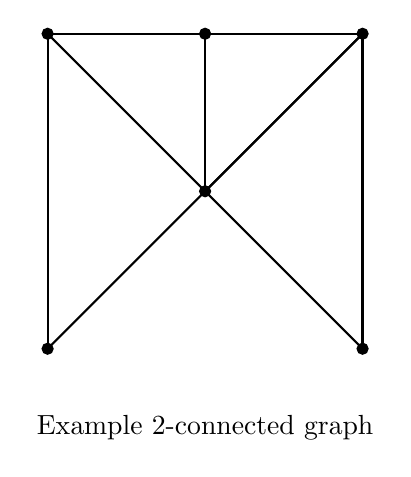
\begin{tikzpicture}
        \draw[black, thick] (0,0) -- (0,4);
        \draw[black, thick] (0,0) -- (4,4);
        \draw[black, thick] (4,0) -- (4,4);
        \draw[black, thick] (2,2) -- (4,4);
        \draw[black, thick] (2,2) -- (2,4);
        \draw[black, thick] (0,4) -- (4,4);
        \draw[black, thick] (0,4) -- (4,0);
        \foreach \x/\y in {0/0, 0/4, 2/2, 2/4, 4/0, 4/4} {
                \filldraw[black] (\x,\y) circle (2pt);
            }
        \node at (2,-1,0) {Example 2-connected graph};
    \end{tikzpicture}
    \hspace{2cm}
    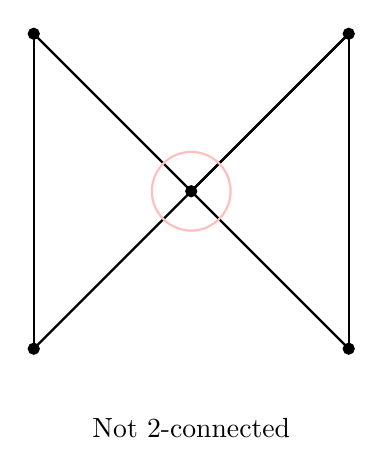
\begin{tikzpicture}
        \draw[black, thick] (0,0) -- (0,4);
        \draw[black, thick] (0,0) -- (4,4);
        \draw[black, thick] (4,0) -- (4,4);
        \draw[black, thick] (2,2) -- (4,4);
        \draw[black, thick] (0,4) -- (4,0);
        \draw[pink, thick] (2,2) circle (0.5);
        \foreach \x/\y in {0/0, 0/4, 2/2, 4/0, 4/4} {
                \filldraw[black] (\x,\y) circle (2pt);
            }
        \node at (2,-1,0) {Not 2-connected};
    \end{tikzpicture}
\end{center}
\begin{theorem}
    Mọi cặp đỉnh trong đồ thị 2-connected đều nằm trên cùng một chu trình.
    \begin{proof}
        Quy nạp:

        Trường hợp cơ bản: $u$ kề $v$
        \begin{center}
            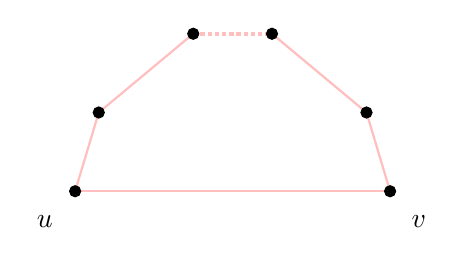
\begin{tikzpicture}
                \draw[pink, thick] (0,0) -- (0.3,1);
                \draw[pink, thick] (0.3,1) -- (1.5,2);
                \draw[densely dotted, pink, ultra thick] (1.5,2) -- (2.5,2);
                \draw[pink, thick] (2.5,2) -- (3.7,1);
                \draw[pink, thick] (3.7,1) -- (4,0);
                \draw[pink, thick] (0,0) -- (4,0);
                \node at (0,0,1) {$u$};
                \node at (4.75,0,1) {$v$};
                \filldraw[black] (0,0) circle (2pt);
                \filldraw[black] (0.3,1) circle (2pt);
                \filldraw[black] (1.5,2) circle (2pt);
                \filldraw[black] (2.5,2) circle (2pt);
                \filldraw[black] (3.7,1) circle (2pt);
                \filldraw[black] (4,0) circle (2pt);
            \end{tikzpicture}
        \end{center}
        Quy nạp: $u,v$ có khoảng cách $d+1$
        \begin{center}
            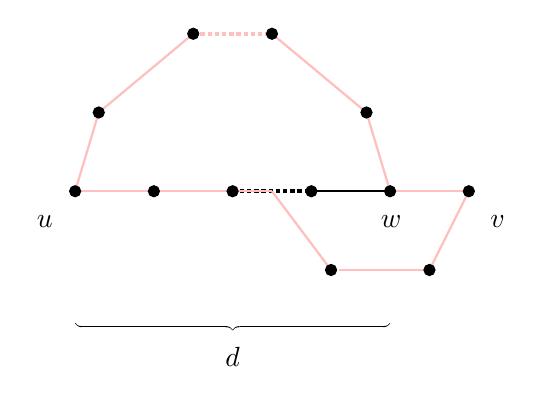
\begin{tikzpicture}
                \draw[pink, thick] (0,0) -- (0.3,1);
                \draw[pink, thick] (0.3,1) -- (1.5,2);
                \draw[densely dotted, pink, ultra thick] (1.5,2) -- (2.5,2);
                \draw[pink, thick] (2.5,2) -- (3.7,1);
                \draw[pink, thick] (3.7,1) -- (4,0);
                \draw[pink, thick] (0,0) -- (2,0);
                \draw[black, thick] (3,0) -- (4,0);
                \draw[pink, thick] (4,0) -- (5,0);
                \draw[densely dotted, black, ultra thick] (2,0) -- (3,0);
                \draw[pink, thick] (2.5,0) -- (3.25,-1);
                \draw[pink, thick] (3.35,-1) -- (4.5,-1);
                \draw[pink, thick] (5,0) -- (4.5,-1);
                \draw[pink, thick] (2,0) -- (2.5,0);

                \node at (0,0,1) {$u$};
                \node at (5.75,0,1) {$v$};
                \node at (4.4,0,1) {$w$};
                \filldraw[black] (0,0) circle (2pt);
                \filldraw[black] (0.3,1) circle (2pt);
                \filldraw[black] (1.5,2) circle (2pt);
                \filldraw[black] (2.5,2) circle (2pt);
                \filldraw[black] (3.7,1) circle (2pt);
                \filldraw[black] (1,0) circle (2pt);
                \filldraw[black] (2,0) circle (2pt);
                \filldraw[black] (3,0) circle (2pt);
                \filldraw[black] (4,0) circle (2pt);
                \filldraw[black] (5,0) circle (2pt);
                \filldraw[black] (3.25,-1) circle (2pt);
                \filldraw[black] (4.5,-1) circle (2pt);

                \draw [decorate, decoration = {calligraphic brace, mirror, raise=5pt}] (0,-1.5) --  (4,-1.5) node[pos=0.5,below=10pt,black]{$d$};
            \end{tikzpicture}
        \end{center}
    \end{proof}
\end{theorem}
\textcolor{blue}{\section{Mã hóa RSA}}
Để mã hóa thông điệp $M$ sử dụng khóa $(n,e)$, trước tiên, ta thay thể chuỗi $M$ bằng chuỗi số nguyên.
Tương tự như mật mã dịch, ta thay mỗi chữ cái bởi mỗi số tương ứng, nhưng khác biệt ở chỗ số được thay là số được biểu diễn bởi 2 chữ số.
Ví dụ A được thay bằng 00, B được thay bằng 01, ..., J được thay bằng 09.
Tiếp theo, ta chia chuỗi vừa thu được thành các khối có độ dài $2N$, trong đó $N$ là số lớn nhất thỏa mãn số 2525...25 có $2N$ chữ số không vượt quá $n$. Ta có thể thêm vào cuối một vài ký tự (nếu cần thiết) để khối cuối cùng có cùng độ dài với các khổi còn lại.

Sau khi thực hiện các bước trên, ta thu được thông điệp $M$ dưới dạng một chuỗi các số nguyên $m_1, m_2, \ldots, m_k$ ($k>0$).
Quá trình mã hóa sẽ chuyển đổi từng khối $m_i$ thành khối mật mã $c_i$ bằng cách sử dụng hàm
$$ c_i = m_i^e\ \mathbf{mod}\ n$$
Ta để thông điệp mã hóa dưới dạng một dãy các khối số và gửi đến
người nhận mà không thay thế các khổi này bằng cách chữ nữa. Bởi vì hệ RSA mã hóa các khối chữ cái thành các
khối ký tự khác, nên nó là một mật mã khối.

Ví dụ 8 minh họa cách thực hiện mã hóa bằng hệ RSA. Để dễ tính toán, trong ví dụ này, $p$ và $q$ là hai số nguyên tố nhỏ thay vì các số nguyên tố có
300 chữ số trở lên, cho nên nó không có tính bảo mật cao.
Mặc dù mật mã trong ví dụ này không an toàn,
nhưng nó minh họa các kỹ thuật được sử dụng trong hệ mã hóa RSA.
\begin{example}
    Mã hóa thông điệp "STOP" dùng hệ RSA với khóa $(n,13),\ p =43,\ q =59$
\end{example}
\begin{solution}
    Vì $n = pq$ nên ta tính được $n=43\times59 = 2537$, chú ý UCLN$(e,(p-1)(q-1)) = 1$.

    Để mã hóa, trước tiên ta thay các chữ cái trong thông điệp bằng các số tương ứng. Sau đó nhóm thành các nhóm có 4 chữ số (vì $2525 < n < 252525$). Ta được
    \begin{center}
        1819 \hspace{0.5cm} 1415
    \end{center}
    Với mỗi khối, ta dùng hàm
    $$ c = m^{13}\ \mathbf{mod}\ 2537$$
    Tính toán cho thấy $1819^{13}\ \mathbf{mod}\ 2537 = 2081$ và $1415^{13}\ \mathbf{mod}\ 2537 = 2182$.
    Thông điệp mã hóa được gửi đi là 2081 2182.
\end{solution}
\section{Proof the Theorem}
The first direction of \hyperref[thr:kuratowski]{Kuratowski's theorem} states: If graph $G$ contains a subdivision of $K_5$ or $K_{3,3}$ then $G$ is nonplanar

Subdivision of Nonplanar is Nonplanar

If a Subgraph is nonplanar then graph is nonplanar

If a subgraph of graph $G$ is a subdivision of nonplanar then $G$ is nonplanar
\begin{lemma}
    $K_{3,3}$ is nonplanar
\end{lemma}

\begin{proof}
    \begin{figure}[H]
        \begin{minipage}{0.3\textwidth}
            $$V-E+F=2$$
            $$6-E+F=2$$
            $$6-9+F=2$$
            $$F=5$$
        \end{minipage}
        \hfill
        \begin{minipage}{0.35\textwidth}
            \centering
            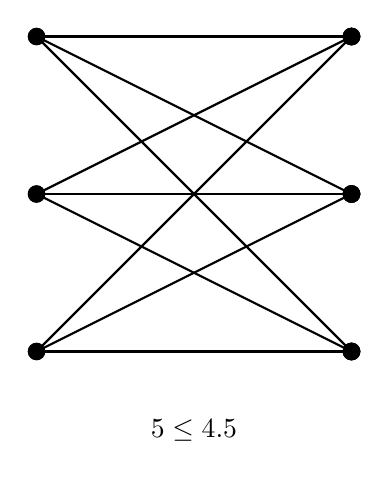
\begin{tikzpicture}
                \foreach \x/\y in {0/1, 0/3, 0/5} {
                        \filldraw[black] (\x,\y) circle (3pt);
                        \foreach \z/\t in {4/1, 4/3, 4/5} {
                                \filldraw[black] (\z,\t) circle (3pt);
                                \draw[black, thick] (\x,\y) -- (\z,\t);
                            }
                    }
                \node at (2,0,0) {$5 \leq 4.5$};
            \end{tikzpicture}
        \end{minipage}
        \hfill
        \begin{minipage}{0.3\textwidth}
            \centering
            No 3 edge faces
            $$4F \leq 2E$$
            $$4F \leq 2 \times 9$$
            $$ F \leq 4.5$$
        \end{minipage}
    \end{figure}
\end{proof}

\begin{lemma}
    $K_5$ is nonplanar
\end{lemma}
\begin{proof}
    \begin{figure}[H]
        \begin{minipage}{0.3\textwidth}
            $$V-E+F=2$$
            $$5-E+F=2$$
            $$5-10+F=2$$
            $$F=7$$
        \end{minipage}
        \hfill
        \begin{minipage}{0.35\textwidth}
            \centering
            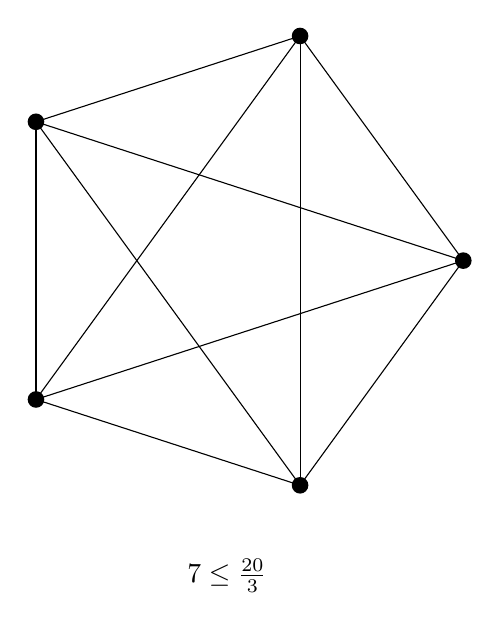
\begin{tikzpicture}
                \foreach \i in {1, 2, 3, 4, 5}
                \fill[black] (\i*360/5:3) coordinate (5\i) circle(3 pt)
                \ifnum \i>1 foreach \j in {\i,...,1}{(5\i) edge (5\j)} \fi;

                \node at (0,-4,0) {$7 \leq \frac{20}{3}$};
            \end{tikzpicture}
        \end{minipage}
        \hfill
        \begin{minipage}{0.3\textwidth}
            \centering
            $$3F \leq 2E$$
            $$3F \leq 2 \times 10$$
            $$F \leq \frac{20}{3}$$
        \end{minipage}
    \end{figure}
\end{proof}
\begin{recap}
    $K_5$ và $K_{3,3}$ are nonplanar

    $\Rightarrow$ All of their subdivisions are nonplanar

    $\Rightarrow$ If graph G contains a subdivision of $K_5$ or $K_{3,3}$ then G is nonplanar
\end{recap}

The second direction of \hyperref[thr:kuratowski]{Kuratowski's theorem} states: If graph $G$ is nonplanar then $G$ contains a subdivision of $K_5$ or $K_{3,3}$
\begin{proof}
    Assume there exist nonplanar graphs which have no subdivisions of $K_5$ or $K_{3,3}$ as subgraphs.

    Let G be the graph of this kind with the $fewest$ edges. Then removing any edge from $G$ gives a $planar$ graph

    \begin{enumerate}
        \item $G$ is 2-connected
              \begin{multicols}{2}
                  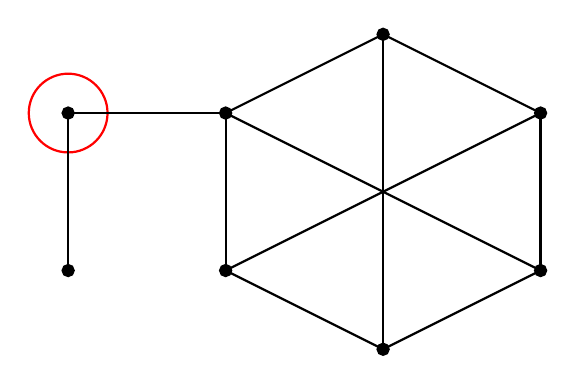
\begin{tikzpicture}
                      \draw[red, thick] (-2,3) circle (0.5);
                      \foreach \x/\y in {0/1, 2/0, 4/1, 0/3, 4/3, 2/4} {
                              \filldraw[black, thick] (\x,\y) circle (2pt);
                              \draw[black, thick] (2,2) -- (\x,\y);
                          }
                      \filldraw[black, thick] (-2,3) circle (2pt);
                      \filldraw[black, thick] (-2,1) circle (2pt);

                      \draw[black, thick] (0,1) -- (2,0);
                      \draw[black, thick] (2,0) -- (4,1);
                      \draw[black, thick] (4,1) -- (4,3);
                      \draw[black, thick] (0,3) -- (0,1);
                      \draw[black, thick] (4,3) -- (2,4);
                      \draw[black, thick] (2,4) -- (0,3);

                      \draw[black, thick] (-2,1) -- (-2,3);
                      \draw[black, thick] (-2,3) -- (0,3);

                  \end{tikzpicture}
              \end{multicols}
        \item $deg(v) \geq 3$ for all vertex $v$ in $G$

              Chứng minh phản chứng: assume some vertex $v \in G$ has $deg(v) \leq 2$

        \item for some $uv \in G$, $G - uv$ is 2-connected
    \end{enumerate}

\end{proof}

Take the egde $uv$ from the previous statement, and consider the graph $G-uv$ obtained by removing it

$G-uv$ is planar by minimality

$G-uv$ is 2-connected, so there is a cycle contains $u,v$.

\begin{remark}
    Note that the edges we are drawing here are really paths in graph
\end{remark}

\begin{figure}[H]
    \begin{minipage}{0.4\textwidth}
        \begin{tikzpicture}
            \draw[black, thick] (0,0) circle (3);
            \filldraw[black, thick] (-3,0) circle (2pt);
            \filldraw[black, thick] (3,0) circle (2pt);
            \node at (-3.5,0,0) {$u$};
            \node at (3.5,0,0) {$v$};
            \node at (0,2.5,0) {$C$};
        \end{tikzpicture}
    \end{minipage}
    \hfill
    \begin{minipage}{0.5\textwidth}
        Embeded maximal cycle $C$ containing $u,v$
    \end{minipage}

\end{figure}

\begin{figure}[H]
    \begin{minipage}{0.4\textwidth}
        \begin{tikzpicture}
            \draw[black, thick] (0,0) circle (3);
            \filldraw[black, thick] (-3,0) circle (2pt);
            \filldraw[black, thick] (3,0) circle (2pt);
            \node at (-3.5,0,0) {$u$};
            \node at (3.5,0,0) {$v$};
            \node at (0,2.5,0) {$C$};
        \end{tikzpicture}
    \end{minipage}
    \hfill
    \begin{minipage}{0.5\textwidth}
        We embeded $G -uv$ so that $C$ enclose more regions of the graph than any other cycle containing $u$ and $v$ could
    \end{minipage}

\end{figure}

\begin{figure}[H]
    \begin{minipage}{0.4\textwidth}
        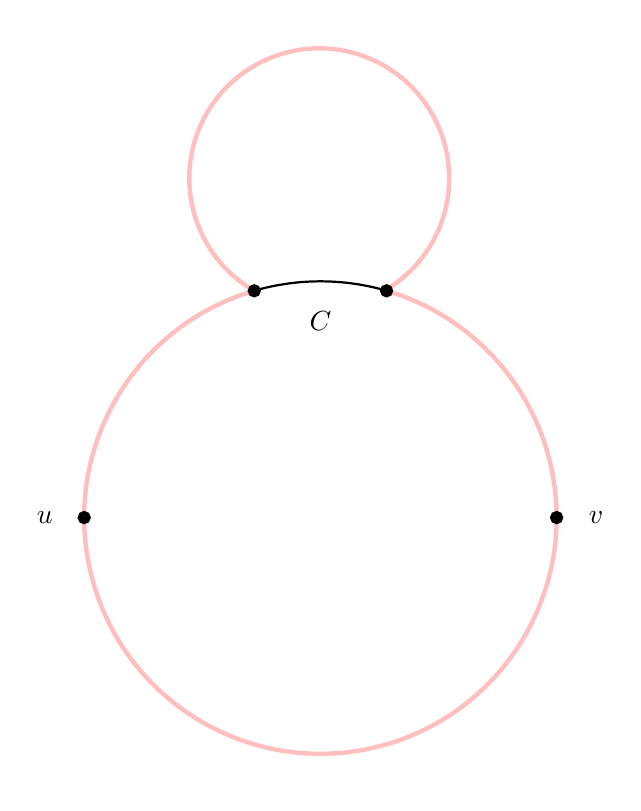
\begin{tikzpicture}
            \draw[black, thick] (0,0) circle (3);
            \draw[pink, ultra thick] (-21/25,72/25) arc (240:-60:1.65);
            \draw[pink, ultra thick] (-21/25,72/25) arc (-253.75:73:3);
            \filldraw[black, thick] (-21/25,72/25) circle (2pt);
            \filldraw[black, thick] (21/25,72/25) circle (2pt);
            \filldraw[black, thick] (-3,0) circle (2pt);
            \filldraw[black, thick] (3,0) circle (2pt);

            \node at (-3.5,0,0) {$u$};
            \node at (3.5,0,0) {$v$};
            \node at (0,2.5,0) {$C$};
        \end{tikzpicture}
    \end{minipage}
    \hfill
    \begin{minipage}{0.4\textwidth}
        Loop along upper or lower part of $C$?

        We can't have any extra paths on the upper or lower part of $C$ since then there would be a cycle which contains more regions

        Larger cycle $\Rightarrow$ Contradiction
    \end{minipage}

\end{figure}


\begin{figure}[H]
    \begin{minipage}{0.4\textwidth}
        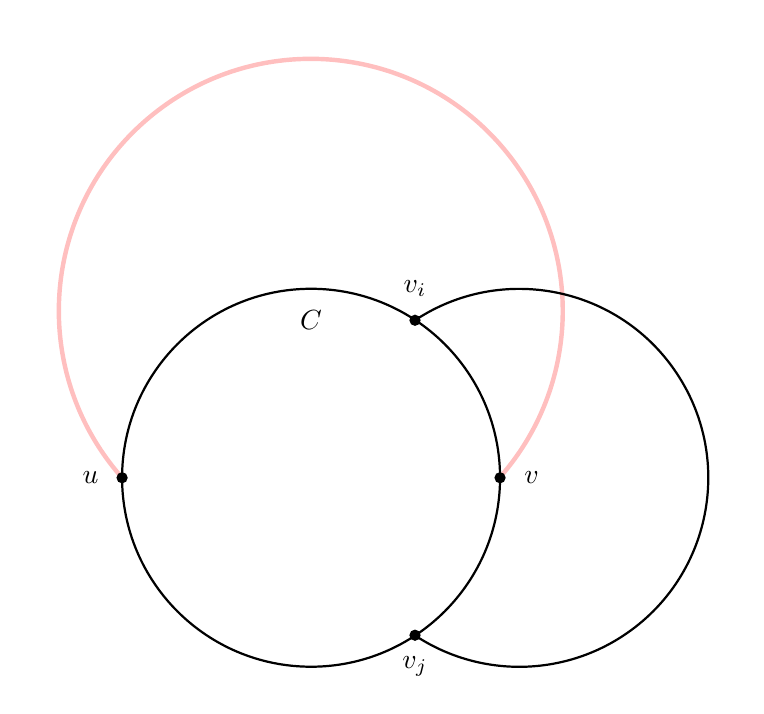
\begin{tikzpicture}[scale = 0.8]
            \draw[black, thick] (0,0) circle (3);
            \draw[pink, ultra thick] (-3,0) arc (221.5:-41:4);
            \draw[black, thick] (1.65,2.5) arc (123.5:-125:3);
            \filldraw[black, thick] (-3,0) circle (2pt);
            \filldraw[black, thick] (3,0) circle (2pt);
            \filldraw[black, thick] (1.65,2.5) circle (2pt);
            \filldraw[black, thick] (1.65,-2.5) circle (2pt);
            \node at (1.65,3,0) {$v_i$};
            \node at (1.65,-3,0) {$v_j$};
            \node at (-3.5,0,0) {$u$};
            \node at (3.5,0,0) {$v$};
            \node at (0,2.5,0) {$C$};
        \end{tikzpicture}
    \end{minipage}
    \hfill
    \begin{minipage}{0.4\textwidth}
        $G$ is nonplanar, so we need an osbtruction to $uv$ on the outside of $C$. There must exist a path $v_iv_j$ that blocks $uv$
    \end{minipage}
\end{figure}

The inside of $C$ must contain an obstruction. This obstruction also has to block $v_iv_j$ from being draw inside of $C$ since otherwise we could just draw it inside and draw $uv$ on the outside.

Up to equivalence there are only four types of obstructions we could draw here. \\

\begin{figure}[H]
    \begin{minipage}{0.4\textwidth}
        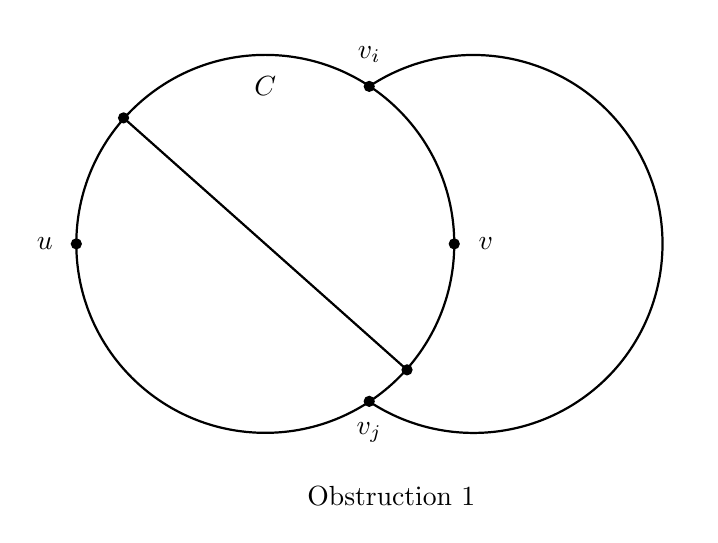
\begin{tikzpicture}[scale = 0.8]
            \draw[black, thick] (0,0) circle (3);
            \draw[black, thick] (1.65,2.5) arc (123.5:-125:3);
            \draw[black, thick] (-2.25,2) -- (2.25,-2);
            \filldraw[black, thick] (-3,0) circle (2pt);
            \filldraw[black, thick] (3,0) circle (2pt);
            \filldraw[black, thick] (-2.25,2) circle (2pt);
            \filldraw[black, thick] (2.25,-2) circle (2pt);
            \filldraw[black, thick] (1.65,2.5) circle (2pt);
            \filldraw[black, thick] (1.65,-2.5) circle (2pt);
            \node at (1.65,3,0) {$v_i$};
            \node at (1.65,-3,0) {$v_j$};
            \node at (-3.5,0,0) {$u$};
            \node at (3.5,0,0) {$v$};
            \node at (0,2.5,0) {$C$};

            \node at (2,-4,0) {Obstruction 1};
        \end{tikzpicture}
    \end{minipage}
    \hfill
    \begin{minipage}{0.4\textwidth}
        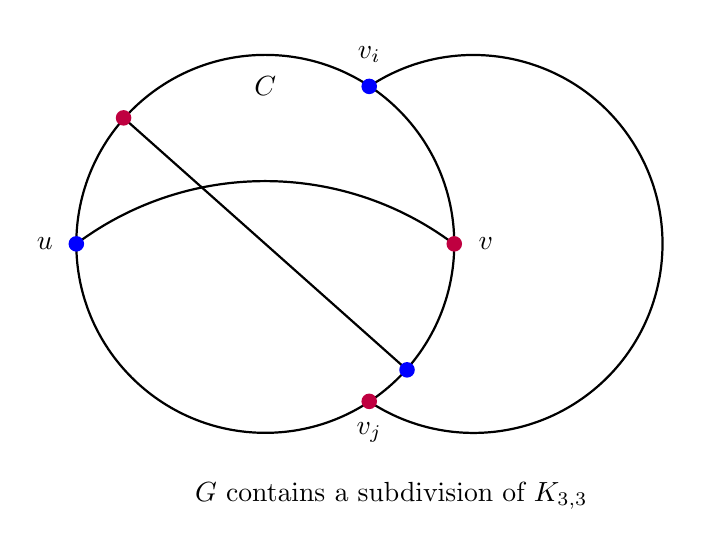
\begin{tikzpicture}[scale = 0.8]
            \draw[black, thick] (0,0) circle (3);
            \draw[black, thick] (1.65,2.5) arc (123.5:-125:3);
            \draw[black, thick] (-3,0) arc (126.8:53:5);
            \draw[black, thick] (-2.25,2) -- (2.25,-2);
            \filldraw[blue, thick] (-3,0) circle (3pt);
            \filldraw[purple, thick] (3,0) circle (3pt);
            \filldraw[purple, thick] (-2.25,2) circle (3pt);
            \filldraw[blue, thick] (2.25,-2) circle (3pt);
            \filldraw[blue, thick] (1.65,2.5) circle (3pt);
            \filldraw[purple, thick] (1.65,-2.5) circle (3pt);
            \node at (1.65,3,0) {$v_i$};
            \node at (1.65,-3,0) {$v_j$};
            \node at (-3.5,0,0) {$u$};
            \node at (3.5,0,0) {$v$};
            \node at (0,2.5,0) {$C$};
            \node at (2,-4,0) {$G$ contains a subdivision of $K_{3,3}$};

        \end{tikzpicture}
    \end{minipage}
\end{figure}

\begin{figure}[H]
    \begin{minipage}{0.4\textwidth}
        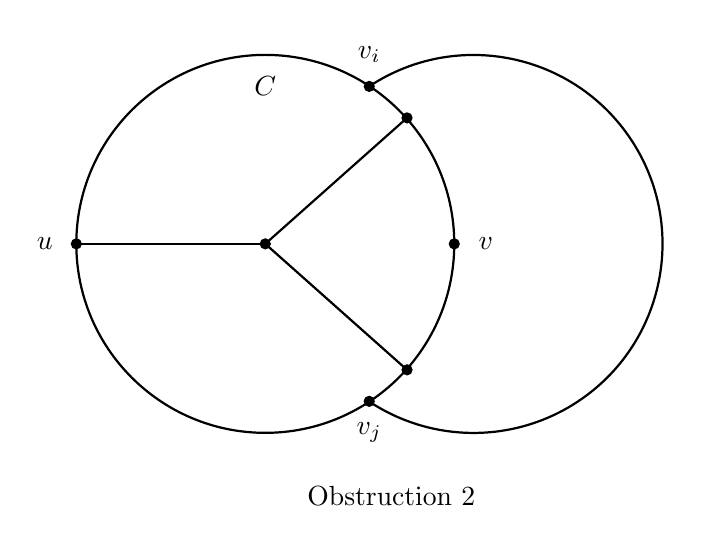
\begin{tikzpicture}[scale = 0.8]
            \draw[black, thick] (0,0) circle (3);
            \draw[black, thick] (1.65,2.5) arc (123.5:-125:3);
            \draw[black, thick] (0,0) -- (2.25,-2);
            \draw[black, thick] (0,0) -- (2.25,2);
            \draw[black, thick] (0,0) -- (-3,0);
            \filldraw[black, thick] (-3,0) circle (2pt);
            \filldraw[black, thick] (3,0) circle (2pt);
            \filldraw[black, thick] (0,0) circle (2pt);
            \filldraw[black, thick] (2.25,2) circle (2pt);
            \filldraw[black, thick] (2.25,-2) circle (2pt);
            \filldraw[black, thick] (1.65,2.5) circle (2pt);
            \filldraw[black, thick] (1.65,-2.5) circle (2pt);
            \node at (1.65,3,0) {$v_i$};
            \node at (1.65,-3,0) {$v_j$};
            \node at (-3.5,0,0) {$u$};
            \node at (3.5,0,0) {$v$};
            \node at (0,2.5,0) {$C$};

            \node at (2,-4,0) {Obstruction 2};
        \end{tikzpicture}
    \end{minipage}
    \hfill
    \begin{minipage}{0.4\textwidth}
        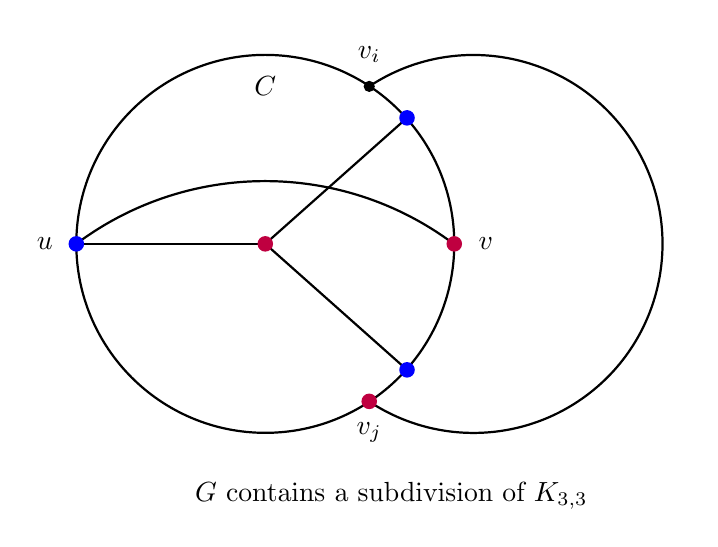
\begin{tikzpicture}[scale = 0.8]
            \draw[black, thick] (0,0) circle (3);
            \draw[black, thick] (1.65,2.5) arc (123.5:-125:3);
            \draw[black, thick] (-3,0) arc (126.8:53:5);
            \draw[black, thick] (0,0) -- (2.25,-2);
            \draw[black, thick] (0,0) -- (2.25,2);
            \draw[black, thick] (0,0) -- (-3,0);
            \filldraw[blue, thick] (-3,0) circle (3pt);
            \filldraw[purple, thick] (3,0) circle (3pt);
            \filldraw[purple, thick] (0,0) circle (3pt);
            \filldraw[blue, thick] (2.25,2) circle (3pt);
            \filldraw[blue, thick] (2.25,-2) circle (3pt);
            \filldraw[black, thick] (1.65,2.5) circle (2pt);
            \filldraw[purple, thick] (1.65,-2.5) circle (3pt);
            \node at (1.65,3,0) {$v_i$};
            \node at (1.65,-3,0) {$v_j$};
            \node at (-3.5,0,0) {$u$};
            \node at (3.5,0,0) {$v$};
            \node at (0,2.5,0) {$C$};
            \node at (2,-4,0) {$G$ contains a subdivision of $K_{3,3}$};

        \end{tikzpicture}
    \end{minipage}
\end{figure}

\begin{figure}[H]
    \begin{minipage}{0.4\textwidth}
        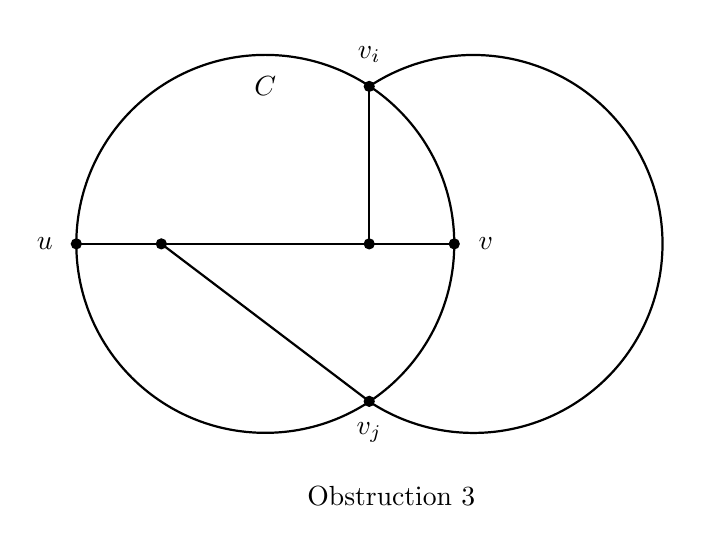
\begin{tikzpicture}[scale = 0.8]
            \draw[black, thick] (0,0) circle (3);
            \draw[black, thick] (1.65,2.5) arc (123.5:-125:3);
            \draw[black, thick] (3,0) -- (-3,0);
            \draw[black, thick] (1.65,0) -- (1.65,2.5);
            \draw[black, thick] (-1.65,0) -- (1.65,-2.5);
            \filldraw[black, thick] (-3,0) circle (2pt);
            \filldraw[black, thick] (3,0) circle (2pt);
            \filldraw[black, thick] (1.65,2.5) circle (2pt);
            \filldraw[black, thick] (1.65,-2.5) circle (2pt);
            \filldraw[black, thick] (1.65,0) circle (2pt);
            \filldraw[black, thick] (-1.65,0) circle (2pt);
            \node at (1.65,3,0) {$v_i$};
            \node at (1.65,-3,0) {$v_j$};
            \node at (-3.5,0,0) {$u$};
            \node at (3.5,0,0) {$v$};
            \node at (0,2.5,0) {$C$};

            \node at (2,-4,0) {Obstruction 3};
        \end{tikzpicture}
    \end{minipage}
    \hfill
    \begin{minipage}{0.4\textwidth}
        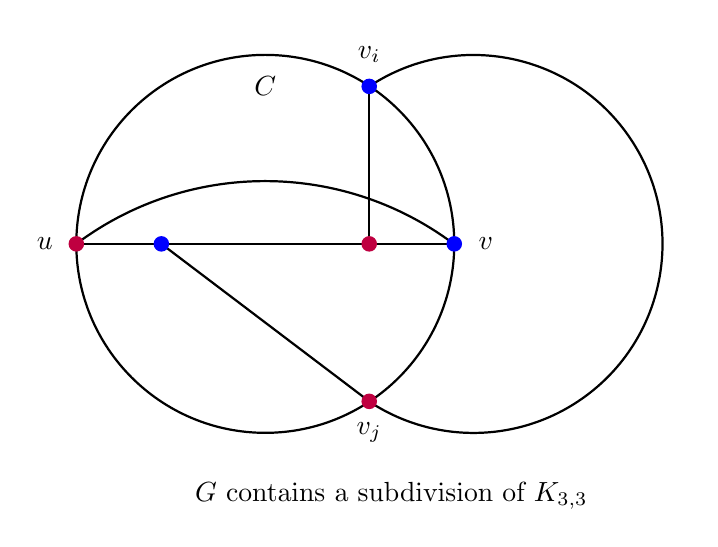
\begin{tikzpicture}[scale = 0.8]
            \draw[black, thick] (-3,0) arc (126.8:53:5);
            \draw[black, thick] (0,0) circle (3);
            \draw[black, thick] (1.65,2.5) arc (123.5:-125:3);
            \draw[black, thick] (3,0) -- (-3,0);
            \draw[black, thick] (1.65,0) -- (1.65,2.5);
            \draw[black, thick] (-1.65,0) -- (1.65,-2.5);
            \filldraw[purple, thick] (-3,0) circle (3pt);
            \filldraw[blue, thick] (3,0) circle (3pt);
            \filldraw[blue, thick] (1.65,2.5) circle (3pt);
            \filldraw[purple, thick] (1.65,-2.5) circle (3pt);
            \filldraw[purple, thick] (1.65,0) circle (3pt);
            \filldraw[blue, thick] (-1.65,0) circle (3pt);
            \node at (1.65,3,0) {$v_i$};
            \node at (1.65,-3,0) {$v_j$};
            \node at (-3.5,0,0) {$u$};
            \node at (3.5,0,0) {$v$};
            \node at (0,2.5,0) {$C$};
            \node at (2,-4,0) {$G$ contains a subdivision of $K_{3,3}$};

        \end{tikzpicture}
    \end{minipage}
\end{figure}


\begin{figure}[H]
    \begin{minipage}{0.4\textwidth}
        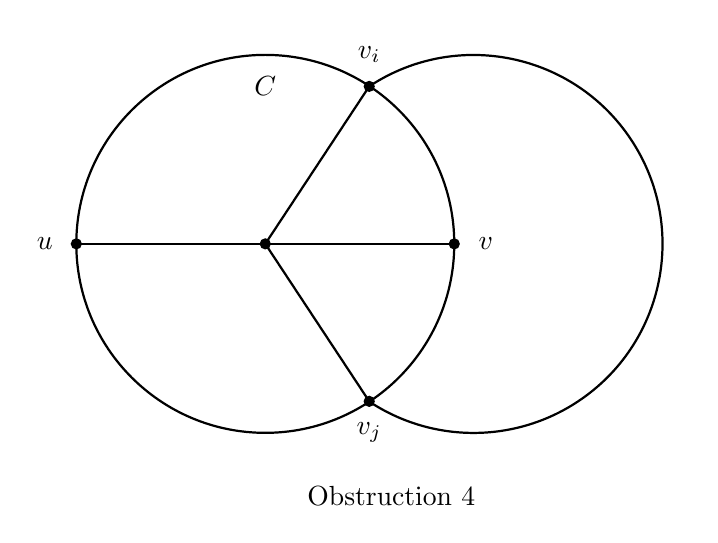
\begin{tikzpicture}[scale = 0.8]
            \draw[black, thick] (0,0) circle (3);
            \draw[black, thick] (1.65,2.5) arc (123.5:-125:3);
            \draw[black, thick] (3,0) -- (-3,0);
            \draw[black, thick] (0,0) -- (1.65,2.5);
            \draw[black, thick] (0,0) -- (1.65,-2.5);
            \filldraw[black, thick] (-3,0) circle (2pt);
            \filldraw[black, thick] (3,0) circle (2pt);
            \filldraw[black, thick] (1.65,2.5) circle (2pt);
            \filldraw[black, thick] (1.65,-2.5) circle (2pt);
            \filldraw[black, thick] (0,0) circle (2pt);
            \node at (1.65,3,0) {$v_i$};
            \node at (1.65,-3,0) {$v_j$};
            \node at (-3.5,0,0) {$u$};
            \node at (3.5,0,0) {$v$};
            \node at (0,2.5,0) {$C$};

            \node at (2,-4,0) {Obstruction 4};
        \end{tikzpicture}
    \end{minipage}
    \hfill
    \begin{minipage}{0.4\textwidth}
        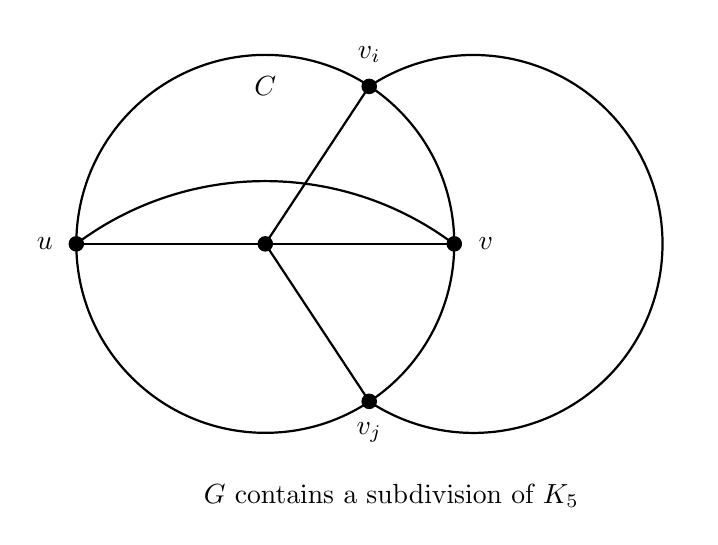
\begin{tikzpicture}[scale = 0.8]
            \draw[black, thick] (-3,0) arc (126.8:53:5);
            \draw[black, thick] (0,0) circle (3);
            \draw[black, thick] (1.65,2.5) arc (123.5:-125:3);
            \draw[black, thick] (3,0) -- (-3,0);
            \draw[black, thick] (0,0) -- (1.65,2.5);
            \draw[black, thick] (0,0) -- (1.65,-2.5);
            \filldraw[black, thick] (-3,0) circle (3pt);
            \filldraw[black, thick] (3,0) circle (3pt);
            \filldraw[black, thick] (1.65,2.5) circle (3pt);
            \filldraw[black, thick] (1.65,-2.5) circle (3pt);
            \filldraw[black, thick] (0,0) circle (3pt);
            \node at (1.65,3,0) {$v_i$};
            \node at (1.65,-3,0) {$v_j$};
            \node at (-3.5,0,0) {$u$};
            \node at (3.5,0,0) {$v$};
            \node at (0,2.5,0) {$C$};
            \node at (2,-4,0) {$G$ contains a subdivision of $K_5$};

        \end{tikzpicture}
    \end{minipage}
\end{figure}
\begin{remark}
    $G$ always contains a subgraph which is subdivisionof $K_5$ or $K_{3,3}$
\end{remark}
In all of the four cases the result is a 4 cases, the result is a contradiction. We assume that $G$ contained at neither of the two graphs. With this, we are left to conclude that there are no nonplanar graphs like $G$. This proves the theorem.


\section*{Acknowledgement}
\addcontentsline{toc}{section}{Acknowledgement}
We would like to thank:
\begin{itemize}
    \item Người hướng dẫn, Nguyen Hai Vinh, vì sự hướng dẫn.
    \item \href{https://cses.fi/book/book.pdf}{Giáo sư Antti Laaksonen} đã giới thiệu chúng tôi đến với Lý thuyết đồ thị.
    \item \href{https://www.youtube.com/channel/UCYO_jab_esuFRV4b17AJtAw}{3Blue1Brown} vì thư viện Python \href{https://github.com/dcabatin/manim}{manim}.
    \item \href{https://www.youtube.com/watch?v=DOnY6eZi2E8}{Nhóm của David Cabatingan} vì những lưu ý về \hyperref[thr:kuratowski]{Định lý Kuratowski}
    \item Ai đấy xây nên cái trường HUS.
\end{itemize}
\end{document}